\section{Research}
First a list of available information that can be achieved from the
mesurement:
\begin{itemize}
  \item the glucose level
  \item the time difference between now and the previous injections
  \item the gradient of the glucose curve at the time of the current measurement
  \item the insulin that will be available in the period p which can be
  calculated as now + ``length of p'' (p can be e.g. 1, 2, 5, 10, 30, \ldots
  minutes or 1, 2, 5, 10, \ldots hours)
  \item the average of the glucose level since a defined point t in the past (t
  has the same definition as p)
\end{itemize}

\subsection{Calculation steps}
\subsubsection{Calculate the gradient (GR) for the current timestamp}
Because of the reason that we don’t have the function of the glucose curve so
that we can derive from we need to calculate the gradient.
One way is to take the gradient from the last and the actual measurement.

\subsubsection{Calculate the available insulin (IN)}
The available insulin can be calculates like in the simulation that you take
the actual timestamp and simply add a period to this time. With the new
timestamp the module insulin and rhe module pangria can calculate the available
insulin for a given period in the future.

\subsubsection{Calculate the actual needed amount of insulin}
As higher GR is as longer the insulin level would increase. Then much more
insulin is needed to get the level down to normal. Than we can calculate with
the amount that is needed to get the glucose level to normal and subtract IN
from this. The result (RE) can be injected.
This is a very simple attempt to calculate the needed amount of insulin.

I assume that we can set a static amount of insulin that will be given by the
pangria. This static amount will be included in the calculation.

\subsection{Further Thoughts}
\begin{itemize}
  \item it is possible to put an factor in front of RE so that just a part of
  the insulin will be injected. The factor depends on GR
  \item we should think about the time period between the measurements to the
  best result
  \item we should define some levels where we put some extra insulin the avoid
  peaks e.g. if we have a big GR but we where in the dangerous area of to less
  sugar then it so problem but if we are in an area where we are already to
  high than is very dangerous
  \item it is possible not to calculate the amount for the future but for the
  past so that we say in the last period the amount of glucose is increased  by
  ``x'' how much insulin is needed to absorb the glucose
  \item in some way we should have a warning in the pump where we inform the
  user if he is in the dangerous area (to high or to low)
\end{itemize}

\section{Analysis Model}

\section{Design Model}
Thanks to the very open and felxible implementation of the Body Simulation
following the Model View Controller (see section \vref{sec:body_simulation})
paradigm, the sensor and injector components of the Insulin pump can be very
easily integrated into the model.

\begin{figure}[htb]
\centering
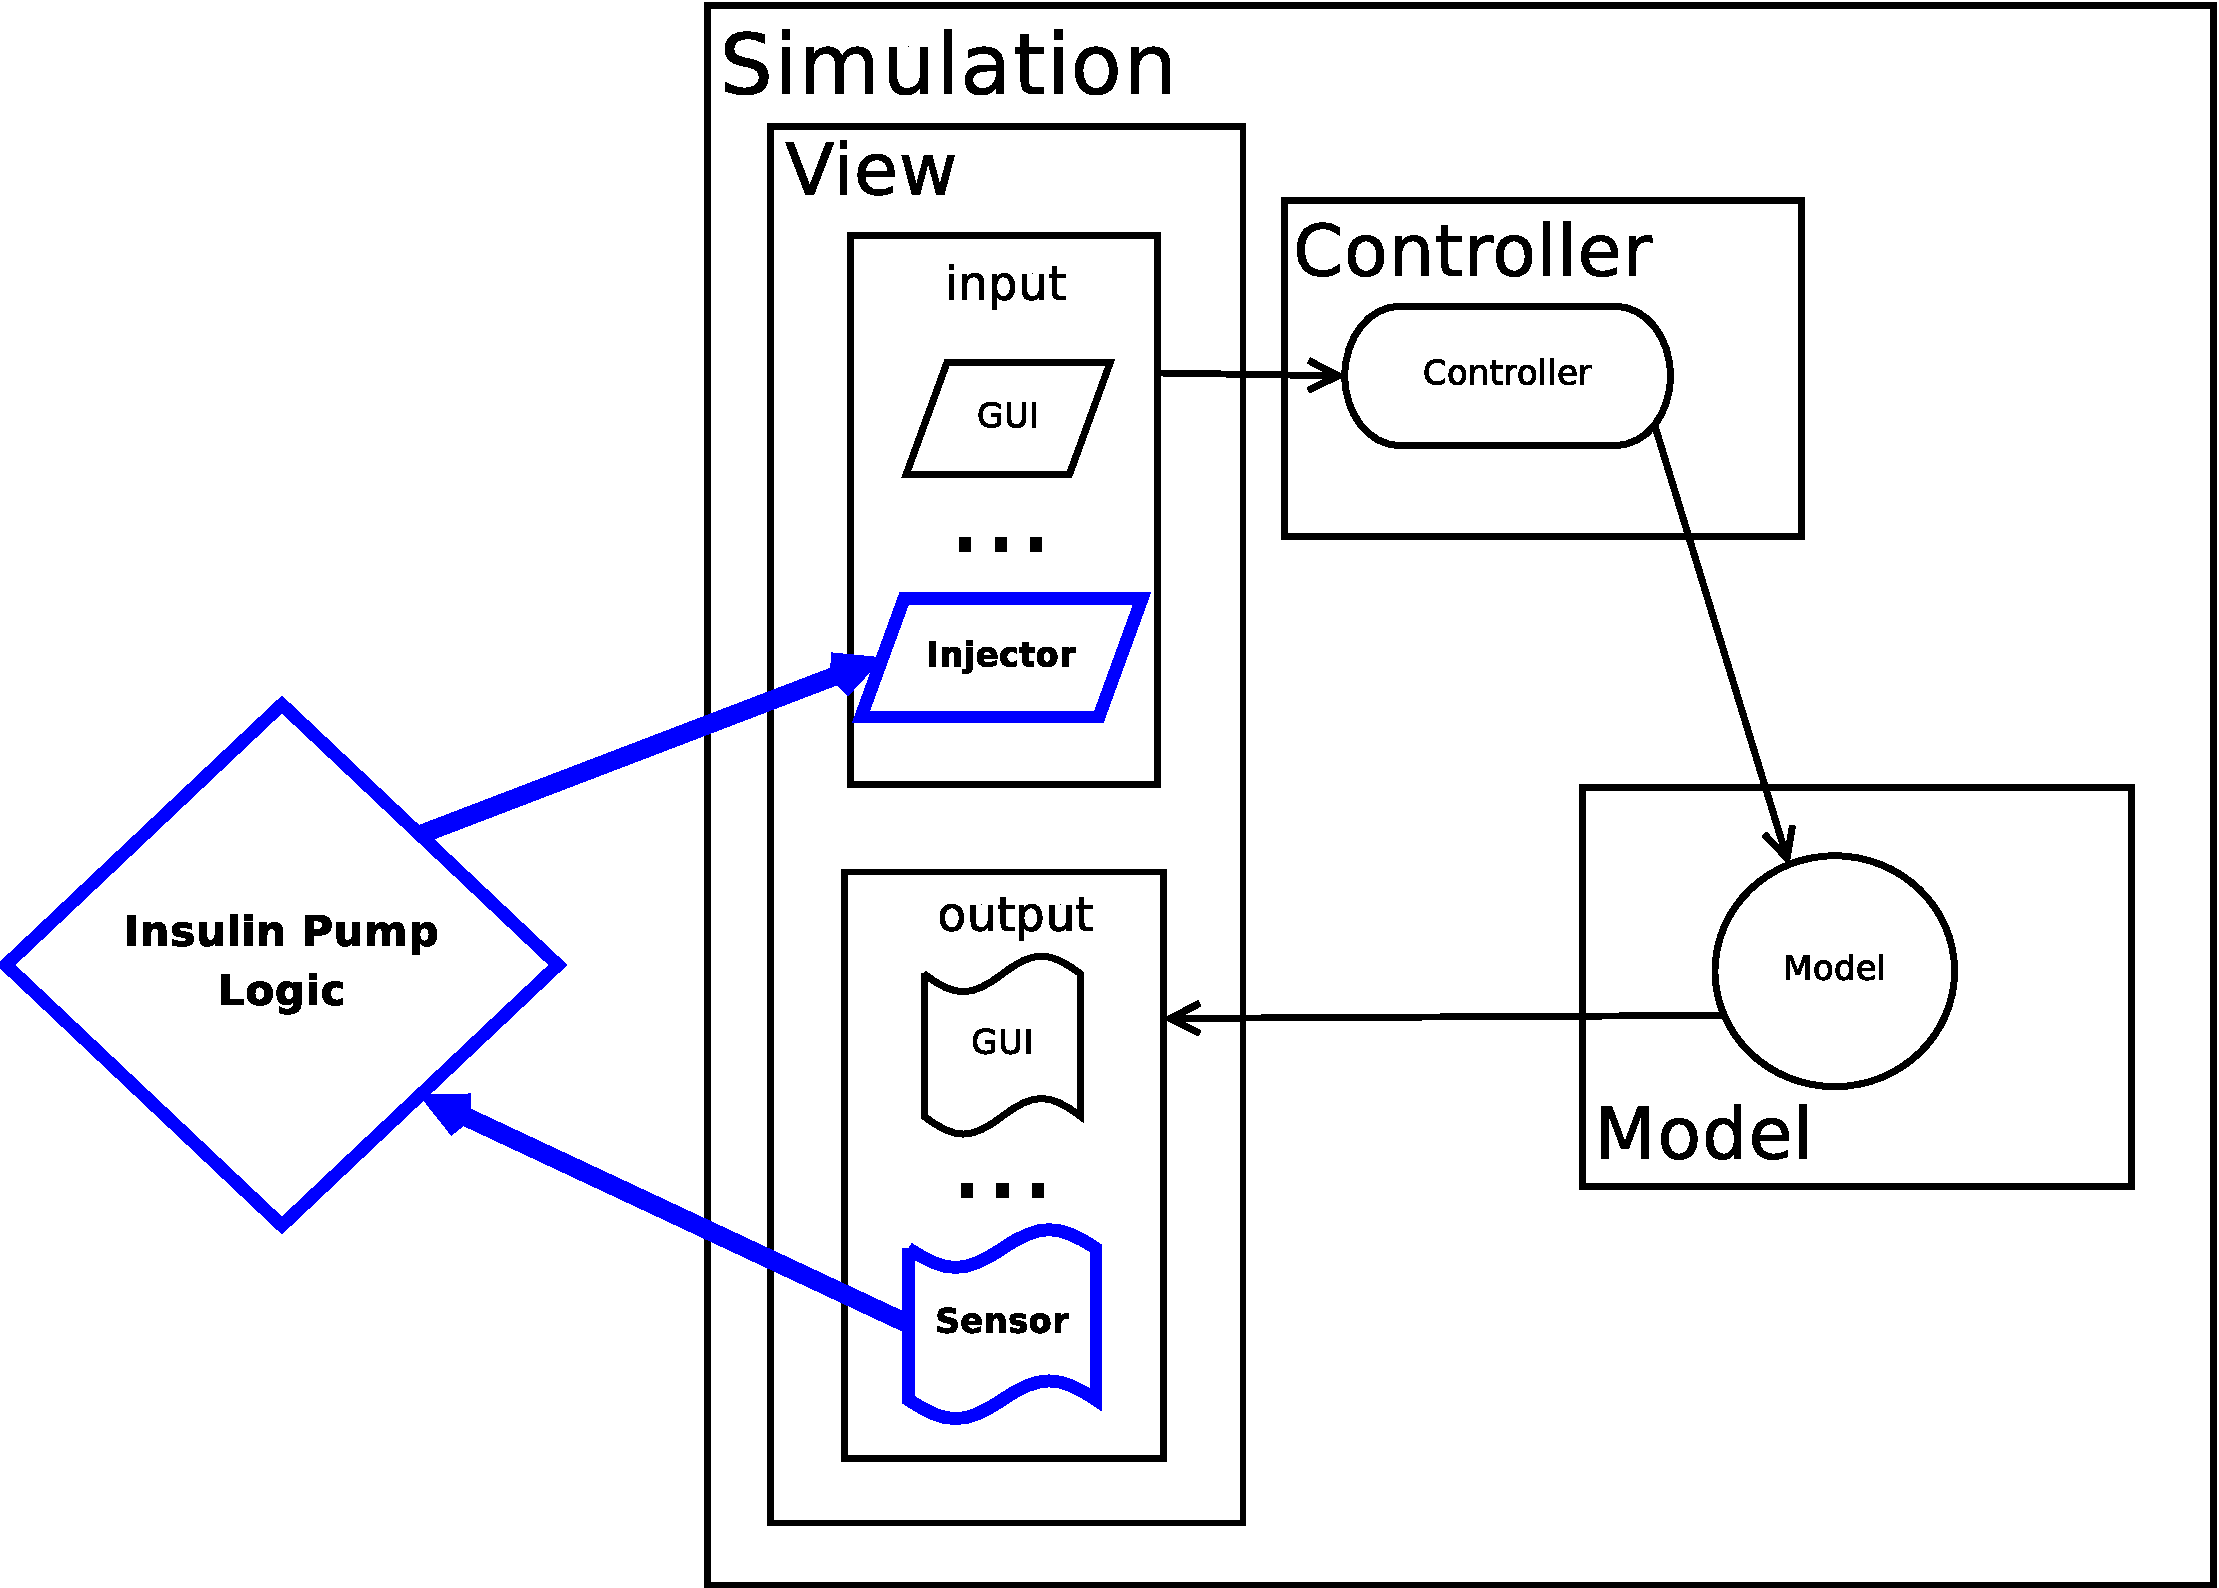
\includegraphics[scale=0.39]{images/mvc_insulin_pump}
\caption{Integration of the Insulin Pump into the Body Simulation}
\label{fig:mvc_insulin_pump}
\end{figure}
